\documentclass[a4paper,12pt]{article}
\usepackage[colorlinks=false,pdfborder=000]{hyperref}
\usepackage[top=1.2in, bottom=1.2in, left=1.2in, right=1.2in]{geometry}
\usepackage[dvips]{graphicx,color}
\usepackage{times}
\usepackage{tikz}
\usepackage{fp}
\usetikzlibrary {snakes,arrows}

%%%%%%%%%%%%%%%%%%%%%%%%%%%%%%%%%%%%%%%%%%%%%%%%%%%%%%%%%%%%%%%%%%
\def\scale{0.7}
\def\half{0.5}
\providecommand{\blockage}[4]{%
    \fill[block] (#1,#2) rectangle (#3+1,#4+1);
}
\providecommand{\drawrowcol}[2]{
    % enumerate the row and column
    \FPset{\row}{#1}
    \FPadd{\row}{\row}{-1}
    \foreach \r in {0,...,\row}
        \node at (0-\half,\r+\half) {\r} ;
    \FPset{\col}{#2}
    \FPadd{\col}{\col}{-1}
    \foreach \c in {0,...,\col}
        \node at (\c+\half,0-\half) {\c} ;
}
\providecommand{\drawgrid}[2]{
    \draw (0,0) grid (#1,#2);
    \drawrowcol{#1}{#2}
}
\providecommand{\drawtwopin}[7]{
%#1= pin1 name #2,#3=pin1 location
%#4= pin1 name #5,#6=pin2 location
%#7= color
    \node[pins,#7]  (#1) at (#2 + \half, #3 + \half) {}; % pin-1
    \node[pins,#7]  (#4) at (#5  + \half, #6 + \half) {}  % pin-2
        edge[arrow] (#1);            % arrow
    %\node[above] at (#1) {$#1$}; % label
    %\node[above] at (#4) {$#4$}; % label
}
\providecommand{\drawthreepin}[9]{
%#1= pin1 name #2,#3=pin1 location
%#4= pin1 name #5,#6=pin2 location
%#7= pin1 name #8,#9=pin3 location
    \node[pins]  (#1) at (#2 + \half, #3 + \half) {}; % pin-1
    \node[pins]  (#4) at (#5  + \half, #6 + \half) {}  % pin-2
        edge[arrow] (#1);            % arrow
    \node[pins]  (#7) at (#8  + \half, #9 + \half) {}  % pin-2
        edge[arrow] (#1);            % arrow
}
%%%%%%%%%%%%%%%%%%%%%%%%%%%%%%%%%%%%%%%%%%%%%%%%%%%%%%%%%%%%%%%%%%
\begin{document}

\begin{figure}
\centering
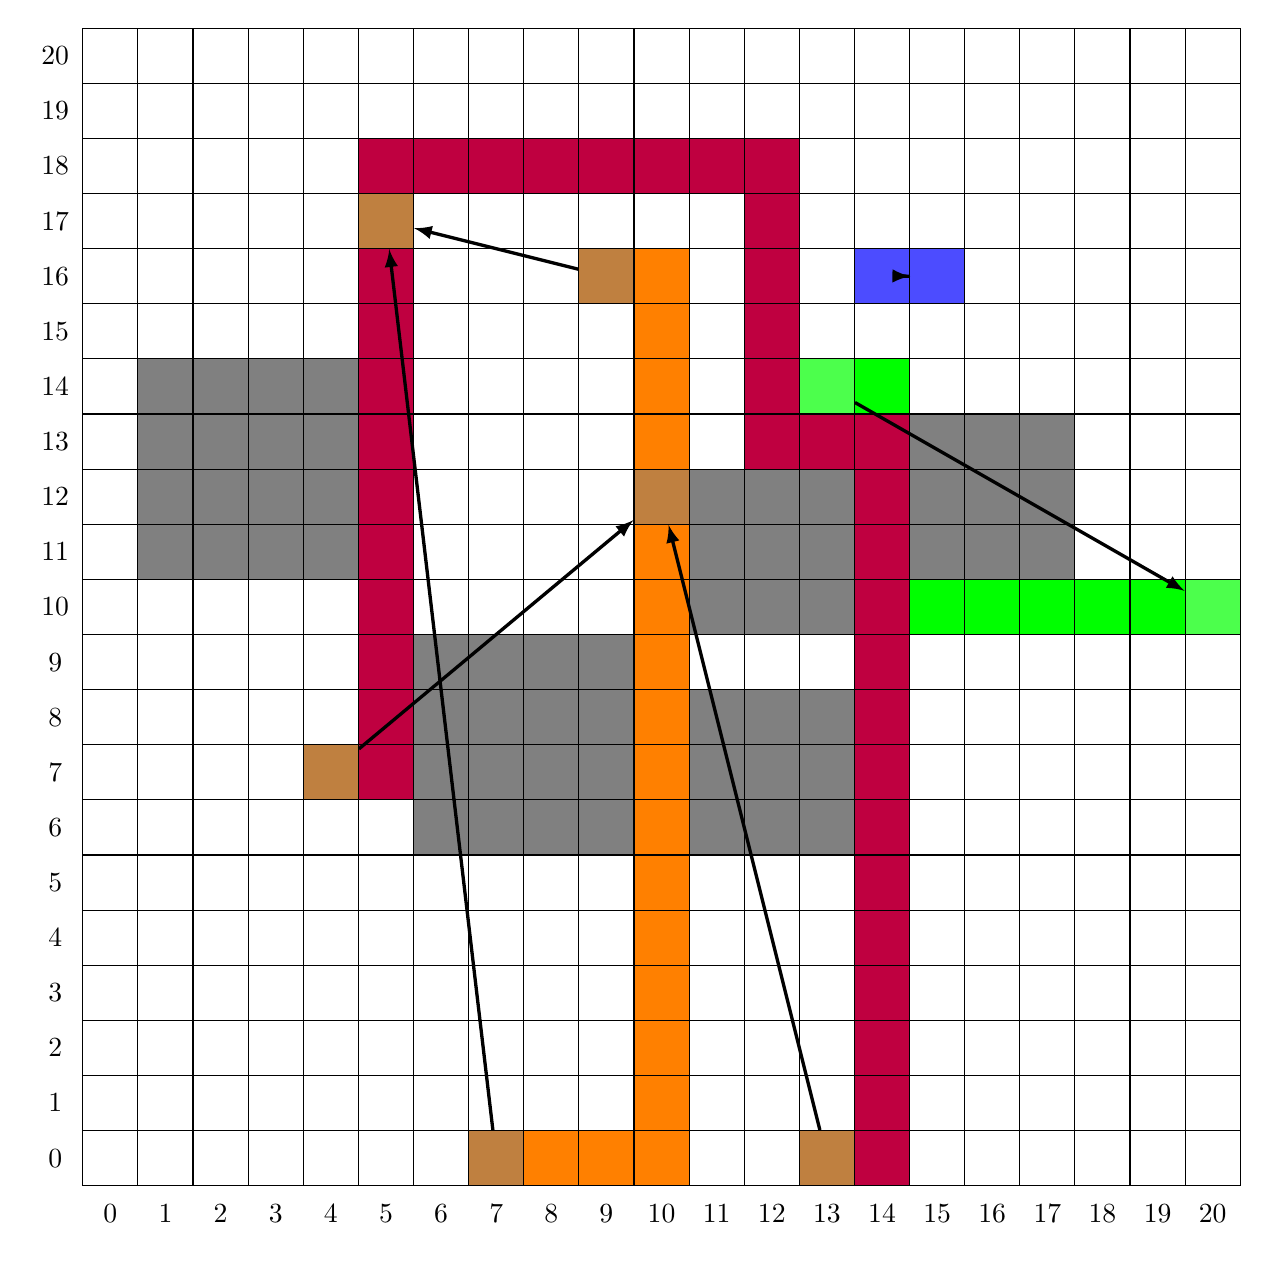
\begin{tikzpicture}[scale=\scale,
	%inner sep=1cm*\scale*\half,
	inner sep=0,
	minimum size=1cm*\scale,
	>=latex,
	pins/.style={rectangle,draw,fill=brown,font=\scriptsize},
	arrow/.style={->,very thick},
	block/.style={gray}]
	% define the row and column number
	\def \N{21}\def \M{21}
	% blockages
	% nets
	
\node[pins,blue] (net_0_14_16) at (14+\half,16+\half) {};
\node[pins,blue] (net_0_15_16) at (15+\half,16+\half) {};

\node[pins,green] (net_1_20_10) at (20+\half,10+\half) {};
\node[pins,green] (net_1_19_10) at (19+\half,10+\half) {};
\node[pins,green] (net_1_18_10) at (18+\half,10+\half) {};
\node[pins,green] (net_1_17_10) at (17+\half,10+\half) {};
\node[pins,green] (net_1_16_10) at (16+\half,10+\half) {};
\node[pins,green] (net_1_15_10) at (15+\half,10+\half) {};
\node[pins,green] (net_1_14_10) at (14+\half,10+\half) {};
\node[pins,green] (net_1_14_11) at (14+\half,11+\half) {};
\node[pins,green] (net_1_14_12) at (14+\half,12+\half) {};
\node[pins,green] (net_1_14_13) at (14+\half,13+\half) {};
\node[pins,green] (net_1_14_14) at (14+\half,14+\half) {};
\node[pins,green] (net_1_13_14) at (13+\half,14+\half) {};

\node[pins,orange] (net_2_9_16) at (9+\half,16+\half) {};
\node[pins,orange] (net_2_10_16) at (10+\half,16+\half) {};
\node[pins,orange] (net_2_10_15) at (10+\half,15+\half) {};
\node[pins,orange] (net_2_10_14) at (10+\half,14+\half) {};
\node[pins,orange] (net_2_10_13) at (10+\half,13+\half) {};
\node[pins,orange] (net_2_10_12) at (10+\half,12+\half) {};
\node[pins,orange] (net_2_10_11) at (10+\half,11+\half) {};
\node[pins,orange] (net_2_10_10) at (10+\half,10+\half) {};
\node[pins,orange] (net_2_10_9) at (10+\half,9+\half) {};
\node[pins,orange] (net_2_10_8) at (10+\half,8+\half) {};
\node[pins,orange] (net_2_10_7) at (10+\half,7+\half) {};
\node[pins,orange] (net_2_10_6) at (10+\half,6+\half) {};
\node[pins,orange] (net_2_10_5) at (10+\half,5+\half) {};
\node[pins,orange] (net_2_10_4) at (10+\half,4+\half) {};
\node[pins,orange] (net_2_10_3) at (10+\half,3+\half) {};
\node[pins,orange] (net_2_10_2) at (10+\half,2+\half) {};
\node[pins,orange] (net_2_10_1) at (10+\half,1+\half) {};
\node[pins,orange] (net_2_10_0) at (10+\half,0+\half) {};
\node[pins,orange] (net_2_9_0) at (9+\half,0+\half) {};
\node[pins,orange] (net_2_8_0) at (8+\half,0+\half) {};
\node[pins,orange] (net_2_7_0) at (7+\half,0+\half) {};

\node[pins,purple] (net_3_4_7) at (4+\half,7+\half) {};
\node[pins,purple] (net_3_5_7) at (5+\half,7+\half) {};
\node[pins,purple] (net_3_5_8) at (5+\half,8+\half) {};
\node[pins,purple] (net_3_5_9) at (5+\half,9+\half) {};
\node[pins,purple] (net_3_5_10) at (5+\half,10+\half) {};
\node[pins,purple] (net_3_5_11) at (5+\half,11+\half) {};
\node[pins,purple] (net_3_5_12) at (5+\half,12+\half) {};
\node[pins,purple] (net_3_5_13) at (5+\half,13+\half) {};
\node[pins,purple] (net_3_5_14) at (5+\half,14+\half) {};
\node[pins,purple] (net_3_5_15) at (5+\half,15+\half) {};
\node[pins,purple] (net_3_5_16) at (5+\half,16+\half) {};
\node[pins,purple] (net_3_5_17) at (5+\half,17+\half) {};
\node[pins,purple] (net_3_5_18) at (5+\half,18+\half) {};
\node[pins,purple] (net_3_6_18) at (6+\half,18+\half) {};
\node[pins,purple] (net_3_7_18) at (7+\half,18+\half) {};
\node[pins,purple] (net_3_8_18) at (8+\half,18+\half) {};
\node[pins,purple] (net_3_9_18) at (9+\half,18+\half) {};
\node[pins,purple] (net_3_10_18) at (10+\half,18+\half) {};
\node[pins,purple] (net_3_11_18) at (11+\half,18+\half) {};
\node[pins,purple] (net_3_12_18) at (12+\half,18+\half) {};
\node[pins,purple] (net_3_12_17) at (12+\half,17+\half) {};
\node[pins,purple] (net_3_12_16) at (12+\half,16+\half) {};
\node[pins,purple] (net_3_12_15) at (12+\half,15+\half) {};
\node[pins,purple] (net_3_12_14) at (12+\half,14+\half) {};
\node[pins,purple] (net_3_12_13) at (12+\half,13+\half) {};
\node[pins,purple] (net_3_13_13) at (13+\half,13+\half) {};
\node[pins,purple] (net_3_14_13) at (14+\half,13+\half) {};
\node[pins,purple] (net_3_14_12) at (14+\half,12+\half) {};
\node[pins,purple] (net_3_14_11) at (14+\half,11+\half) {};
\node[pins,purple] (net_3_14_10) at (14+\half,10+\half) {};
\node[pins,purple] (net_3_14_9) at (14+\half,9+\half) {};
\node[pins,purple] (net_3_14_8) at (14+\half,8+\half) {};
\node[pins,purple] (net_3_14_7) at (14+\half,7+\half) {};
\node[pins,purple] (net_3_14_6) at (14+\half,6+\half) {};
\node[pins,purple] (net_3_14_5) at (14+\half,5+\half) {};
\node[pins,purple] (net_3_14_4) at (14+\half,4+\half) {};
\node[pins,purple] (net_3_14_3) at (14+\half,3+\half) {};
\node[pins,purple] (net_3_14_2) at (14+\half,2+\half) {};
\node[pins,purple] (net_3_14_1) at (14+\half,1+\half) {};
\node[pins,purple] (net_3_14_0) at (14+\half,0+\half) {};
\node[pins,purple] (net_3_13_0) at (13+\half,0+\half) {};

\blockage{1}{11}{4}{14}
\blockage{6}{6}{9}{9}
\blockage{11}{6}{13}{8}
\blockage{11}{10}{13}{12}
\blockage{15}{11}{17}{13}
\drawtwopin{Dlt36_to_Mix05}{14}{16}{Dlt36}{15}{16}{blue!70}
\drawtwopin{W}{20}{10}{Dlt36}{13}{14}{green!70}
\drawthreepin{Mix03}{5}{17}{Dlt34_to_Mix03}{9}{16}{R1}{7}{0}
\drawthreepin{Mix04}{10}{12}{Dlt35_to_Mix04}{4}{7}{R2}{13}{0}
\drawgrid{\N}{\M}
	\end{tikzpicture}
      \end{figure}
      \end{document}
